\chapter{Architecture of Pb\_Multiphase}
This chapter aims to describe how the software is programmed and managed within the TrioCFD/TRUST and physical framework. We first present the numerical problems available (section \ref{archi:problem}), which then give rise to a numerical description of the system of equations presented in section \ref{archi:equation}. This system is stored in matrices, whose filling principle is described in the section \ref{archi:matrix}. The various code storage locations are explained in the section \ref{archi:folder}. Finally, a description of the TrioCFD multiphase GUI prototype for beginners is proposed in section \ref{archi:GUI}.
\section{The problem}\label{archi:problem}
In order to launch the most efficient and suitable numerical simulation possible, it is important to specify what type of equation system one wishes to use. This is referred to as a Problem (Pb) in TRUST/TrioCFD. This Problem is equivalent to a module in other CFD codes. Thus, depending on the type of Problem chosen, different sets of equations are obtained, solved over the domain, so it is crucial to choose it correctly. The different Problems are documented in the Trust Reference Manual at https://cea-trust-platform.readthedocs.io/en/latest/.\\
TrioCFD multiphase corresponds to the multiphase averaged Euler-Euler equation set for motion. Two types of problems are currently available:
\begin{itemize}
\item[\small \textcolor{blue}{\ding{109}}] \texttt{Pb_multiphase} : it allows solving N-phases with a set of 3*N equations (mass, energy, and momentum for each phase). This modeling corresponds to the Two-fluid described in section \ref{sec:two-fluid-drift}. 
\item[\small \textcolor{blue}{\ding{109}}] \texttt{Pb_multiphase_HEM} : it allows solving 2 mechanically and thermally coupled phases at equilibrium via a single set of 3 equations (mass, energy, and momentum for the mixture). This modeling corresponds to the Drift flux with thermal equilibrium described in section \ref{sec:two-fluid-drift}.
\end{itemize}
\texttt{Pb_multiphase_HEM} is notably a reduction of the Pb_multiphase system via an operator called Evanescence, described in section \ref{sec:evanescence}. The use of this problem is equivalent to adding the following line to the data set in a \texttt{Pb_multiphase} :
\begin{lstlisting}[language=c++]
evanescence { homogene { alpha_res 1 alpha_res_min 0.5 } }
\end{lstlisting}
\section{The equations}\label{archi:equation}
Here is a description of the structure of \texttt{Pb_multiphase} set of equations in the code.\\
A structural hypothesis is that the sum of void fractions $\alpha_k$ is such that (see equation \ref{base:contaxiom}):
\begin{equation}
    \sum _k \alpha_k = 1 \label{eq:sumalpha}
\end{equation}
Then, the governing equations of the model used in Pb_multiphase can be written as (refer to equations \ref{base1:1}, \ref{base2:1} and \ref{base2:2} respectively for mass, momentum and energy equations): 
\begin{align}
  & (\mathcal{M}_k) && \frac{\partial  \alpha_k \rho_k}{\partial t} + \underbrace{\nabla \cdot ({\alpha_k \rho_k} \vec{u_k})}_\text{{\colorbox{codebackground}{\color{codekeyword3} convection}}}
                       = \underbrace{\Gamma_k}_\text{ {\colorbox{codebackground}{\color{codekeyword3} sources}}} \label{eq:edpMk}\\
  & (\mathcal{Q}_k) &&
                       \begin{multlined}[c][0.8\linewidth]
                         \frac{\partial \alpha_k \rho_k \vec{u_k}}{\partial t} + \underbrace{\underline{\nabla} \cdot \parent{{\alpha_k \rho_k \vec{u_k}} \otimes \vec{u_k}}}_\text{{\colorbox{codebackground}{\color{codekeyword3} convection}}} = \underbrace{- \ \alpha_k \underline{\nabla} P}_\text{{\colorbox{codebackground}{\color{codekeyword3} solveur_pression}}}
                         + \underbrace{\underline{\nabla} \cdot (\alpha_k \mu_k \underline{\underline{\nabla}} \vec{u_k})}_\text{{\colorbox{codebackground}{\color{codekeyword3} diffusion}}}
                         \\- \underbrace{ \underline{\nabla} \cdot  (\alpha_k\rho_k \overline{u_i'u_j'})}_\text{ {\colorbox{codebackground}{\color{codekeyword3} diffusion}}}
                         + \underbrace{\vec{F}_{ki} + \vec{F}_k}_\text{ {\colorbox{codebackground}{\color{codekeyword3} sources}}}
                       \end{multlined}\label{eq:edpQk}\\
  &(\mathcal{E}_k) &&
                      \begin{multlined}[c][0.8\linewidth]
                        \frac{\partial \alpha_k \rho_k e_k}{\partial t} + \underbrace{\nabla \cdot \parent{{\alpha_k \rho_k e_k} \vec{u_k}}}_\text{{\colorbox{codebackground}{\color{codekeyword3} convection}}}
                        =
                        \underbrace{\nabla \cdot \parent{\alpha_k\lambda_k \underline{\nabla} T - \alpha_k\rho_k \overline{u_i'e_k'}}}_{\text{{\colorbox{codebackground}{\color{codekeyword3} diffusion}}}}
                        \\ -\underbrace{p \parent{\frac{\partial \alpha_k}{\partial t} + \nabla \cdot (\alpha_k \overline{u_k})}}_{\text{{\colorbox{codebackground}{\color{codekeyword3} sources}}}} +
                        \underbrace{q_{ki} + q_{kp}}_{\text{ {\colorbox{codebackground}{\color{codekeyword3} sources}}}}
                      \end{multlined}\label{eq:edpEk}
\end{align}

\begin{table}[!ht]
\begin{center}
\renewcommand{\arraystretch}{2}
   \begin{tabular}{ c  c  c  c }
     \toprule
     Equation & Mass & Momentum & Energy \\
     \midrule
     Keyword  & {\colorbox{codebackground}{\color{codekeyword2} Masse_Multiphase}} & {\colorbox{codebackground}{\color{codekeyword2} QDM_Multiphase}} & {\colorbox{codebackground}{\color{codekeyword2} Energie_Multiphase}} \\
     Abbreviations & $(\mathcal{M}_k)$ & $(\mathcal{Q}_k)$  &  $(\mathcal{E}_k)$  \\
     Unknown & $\alpha_k$ & $p$,$\overrightarrow{u_k} $  & $T$\\
     Conservation & $\rho_k\alpha_k$ & $\rho_k\alpha_k \overrightarrow{u_k} $  & $\rho_k\alpha_k e_k$ \\
     Operators & {\colorbox{codebackground}{\color{codekeyword3} convection}} & \makecell{{\colorbox{codebackground}{\color{codekeyword3} convection}},{\colorbox{codebackground}{\color{codekeyword3} diffusion}},\\ {\colorbox{codebackground}{\color{codekeyword3} solveur_pression}}} & {\colorbox{codebackground}{\color{codekeyword3} convection}}, {\colorbox{codebackground}{\color{codekeyword3} diffusion}} \\
     \bottomrule
   \end{tabular}
 \end{center}
 \caption{Solved equations in TrioCFD multiphase module.}
\label{tab:schema}
\end{table}
 A conservation equation can be seen as a time-change term for a conserved quantity varying according to the physical models we use (see equation \ref{base:everything}). Among those models are convection, diffusion, and source terms. Thus, in the code, an equation corresponds to a time-dependent term for a conserved quantity. It is then associated with keywords allowing to fill in the equation. This is the case for the previous equations \ref{eq:edpMk}, \ref{eq:edpQk} and  \ref{eq:edpEk}, where the conserved quantities and the models are  partially given in Table \ref{tab:schema}.

\subsection{The correlation block and sources}
The correlation bloc contains the list of all closure laws and models for the right-hand side of the equation that can be used in the equations as sources. Thus, all terms that are not related to {\color{codekeyword3} convection} or {\color{codekeyword3} diffusion} or {\color{codekeyword3} solveur_pression} of the conserved field must inherit from \texttt{Correlation_base}.\\
Once notified in the correlation block, the models can be used as a source for the equations. The source terms are semi-implicit to manage the method's tables, notably the availability of derivative calculation during the method. The only purely implicit term is interfacial friction. Regarding time resolution methods described in section \ref{sec:time_scheme}, it should be noted that in ICE/SETS, all other terms are semi-implicit. In PAT, all terms are implicit except for turbulent dispersion due to the void fraction gradient.

\subsection{Turbulent viscosity}
It is a \texttt{Correlation_base}. The value turbulent viscosity field is filled with the \texttt{eddy viscosity} method. If we want to use a more complex form, we can use the Viscosite_turbulente_multiple which uses the reynolds\textunderscore stress method. It is used by the WIT, WIF or sato model, described in section \ref{subsec:RSM}. It might be useful to generalise this to the Visco\textunderscore turbu\textunderscore base.
%%%
\section{Principle of matrix filling}\label{archi:matrix}
The implementation of new source terms is based on the principle of filling partial derivative matrices using the chain rule method. The chain rule is a fundamental concept in calculus that allows us to find the derivative of a composite function. It is particularly useful when dealing with functions of several variables.
Consider a function $f\left(x_1,x_2,\ldots,x_n\right)$ which depends on $n$ variables. If each of these variables $x_i$ depends on another variable $t$, i.e. $x_i=g_i\left(t\right)$, then we can define a composite function $F\left(t\right)=f\left(g_1\left(t\right),g_2\left(t\right),\ldots,g_n\left(t\right)\right)$. Then we can compute an infinitesimal change $dF$ as:
\begin{equation}
dF = \sum_i \frac{\partial F}{\partial g_i} \delta g_i
\end{equation}
The chain rule describes how variations in the independent variable t are transmitted through the dependent variables $x_i$, ultimately influencing changes in the composite function F.
In our case $F(t)=f\parent{\alpha(t), T(t), P(t), \vec{u}(t)}$. We then have: 
\begin{equation}
dF=\frac{\partial F}{\partial \alpha} \delta \alpha +  \frac{\partial F}{\partial P} \delta P + \frac{\partial F}{\partial T} \delta T + \frac{\partial F}{\partial \vec{u}} \delta \vec{u}
\end{equation}
This gives us how to fill respectively the void fraction, temperature, pressure and velocity dependance matrices $M_\alpha$, $M_{T}$, $M_{P}$ and $M_u$ and the right-hand side of the equation (called \texttt{secmem} in the code, French for RHS) so that: 
\begin{equation}
F^{n+1}=\underbrace{F^{n}}_{\text{secmem}} + \underbrace{\frac{\partial F}{\partial \alpha}}_{-M_\alpha} \delta \alpha +  \underbrace{\frac{\partial F}{\partial P}}_{-M_{P}} \delta P +\underbrace{ \frac{\partial F}{\partial T}}_{-M_{T}} \delta T + \underbrace{\frac{\partial F}{\partial \vec{v}}}_{-M_{u}} \delta \vec{u}
\end{equation}
For example, we can consider the pressure term in the energy equation \ref{eq:edpEk}. Its expression is :
\begin{equation}
    -P\parent{\frac{\partial \alpha_k}{\partial t}+\nabla \cdot (\alpha_k u_k)}
\end{equation}
Regarding the temporal change $P\frac{\partial \alpha}{\partial t}$ (similar for the divergence but easier to write here), if we perform the chain rule, one can get :
\begin{itemize}
    \item[\small \textcolor{blue}{\ding{109}}] $F^n=P^n\frac{\Delta \alpha}{\Delta t}$,
    \item[\small \textcolor{blue}{\ding{109}}] $\frac{\partial F}{\partial \alpha}=P^n\frac{1}{\Delta t}$
    \item[\small \textcolor{blue}{\ding{109}}] $\frac{\partial F}{\partial P}=\frac{\Delta \alpha}{\Delta t}$,
    \item[\small \textcolor{blue}{\ding{109}}] $\frac{\partial F}{\partial T}=0$,
    \item[\small \textcolor{blue}{\ding{109}}] $\frac{\partial F}{\partial u}=0$.
\end{itemize}
Then, we can fill the matrix. We add in the right-hand side of the energy equations :
\begin{equation}
    \texttt{secmem}=-P^n \times \frac{\alpha_k^n-\alpha_k^{n-1}}{\Delta t}
\end{equation}
In the void fraction matrix :
\begin{equation}
    M_\alpha=\frac{P^n}{\Delta t}
\end{equation}
In the pressure matrix :
\begin{equation}
    M_P=\frac{\alpha_k^n-\alpha_k^{n-1}}{\Delta t}
\end{equation}
In the energy equation, it means that this term is :
\begin{equation}
M_T=-P^n \times \frac{\alpha_k^n-\alpha_k^{n-1}}{\Delta t}-\frac{\alpha_k^n-\alpha_k^{n-1}}{\Delta t}\delta P - \frac{P^n}{\Delta t}\delta \alpha_k 
\end{equation}
Let's introduce $\alpha_k^n-\alpha_k^{n-1}=\Delta \alpha_k$ and remind that $\delta P =P^{n+1}-P^n$. We then have :
\begin{equation}
-P^n \times \frac{\Delta \alpha_k}{\Delta t}-\frac{\Delta \alpha_k}{\Delta t}(P^{n+1}-P^n) - \frac{P^n}{\Delta t}\delta \alpha_k = -P^{n+1}\frac{\Delta \alpha_k}{\Delta t}-P^n\frac{\delta \alpha_k}{\Delta t} \thicksim -(P\frac{\partial \alpha_k}{\partial t})^{n+1}
 \end{equation}

\subsection*{\color{red} Warning pressure reduction}
Not all dependencies are allowed. Indeed, in order to perform pressure reduction, it is mandatory to keep empty matrices for dependencies on $\alpha$ and T. Thus, if the source term F is in the momentum conservation equation, it can only depend on velocity and pressure $F(P,\vec{u})$ (see Tchen force). In summary :
\begin{itemize}
\item[\small \textcolor{blue}{\ding{109}}] In mass equation (with the unknown $\alpha$), $F(\alpha, T, P, \vec{u})  \Leftrightarrow (M_\alpha,M_T, M_P,M_u)$ filling
\item[\small \textcolor{blue}{\ding{109}}] In energy equation (with the unknown $T$), $F(\alpha, T, P, \vec{u}) \Leftrightarrow (M_\alpha,M_T, M_P,M_u)$ filling
\item[\small \textcolor{blue}{\ding{109}}] In momentum equation (with the unknown $\vec{v}$), $F(P, \vec{u}) \Leftrightarrow (M_P,M_u)$ filling otherwise no pressure reduction allowed.
\end{itemize}
Furthermore, only dependence matrices $M_p$ and $M_u$ (except in momentum equation for the velocity) can be filled with non diagonal terms. In other words, $M_\alpha$ and $M_T$ are always diagonal for all transported variables (including turbulence and diameter) and $M_u$ in the momentum equation is always diagonal.

\section{Folder structure}\label{archi:folder}
The software inherits the complex structure of TrioCFD, which shares part of its source code with TRUST. The aim of this section is to describe the distribution of lines of code linked to TrioCFD multiphase.
TrioCFD multiphase is structured into 2 parts. The first part inherits the structuring of the CFD codes from CEA with the TRUST base. The \texttt{Pb_multiphase}  from TRUST is common to several CEA codes as depicted in Figure \ref{Blocs}.
\begin{figure}[!ht]
    \centering
    \begin{tikzpicture}
        \draw[fill=mydarkorchid!40] (0,0) rectangle (15,1); 
        \node[align=center] at (7.5,0.5) {Trust/Pb_multiphase};
        \draw[fill=mycrimson!50] (0,1) rectangle ++(2.5,1.1);
        \node[align=center] at (1.25,1.5) {TrioCFD};
        \draw[fill=myorange!50] (2.5,1) rectangle ++(2.5,1.1);
        \node[align=center] at (3.75,1.5) {CATHARE3};
        \draw[fill=mygoldenrod!50] (5,1) rectangle ++(2.5,1.1);
        \node[align=center] at (6.25,1.5) {FLICA5};
        \draw[fill=mygreen!50] (7.5,1) rectangle ++(2.5,1.1);
        \node[align=center] at (8.75,1.5) {GENEPI+};
        \draw[fill=myteal!50] (10,1) rectangle ++(2.5,1.1);
        \node[align=center] at (11.25,1.5) {TrioMC};
        \draw[fill=myslateblue!50] (12.5,1) rectangle ++(2.5,1.1);
        \node[align=center] at (13.75,1.5) {SCONE};
    \end{tikzpicture}
    \caption{\texttt{Pb_multiphase} and its baltiks.}
    \label{Blocs}
\end{figure}
The specific parts of TrioCFD multiphase is located in the TrioCFD and Trust folders. The different parts are structured as follows:\\
\begin{forest}
  for tree={
    font=\ttfamily,
    grow'=0,
    edge path={
      \noexpand\path [draw, \forestoption{edge}] (!u.parent anchor) -- +(5pt,0) |- (.child anchor)\forestoption{edge label};
    },
    parent anchor=east,
    child anchor=west,
    anchor=west,
    before typesetting nodes={
      if n=1
        {insert before={[,phantom]}}
        {}
    },
    fit=band,
    s sep=10pt,
    inner sep=2pt,
  }
  [$\thicksim$/,
    [TRUST/src/ThHyd/Multiphase
      [\color{mycrimson} Correlations]
      [\color{myorange} Equations]
      [\color{mygoldenrod} Milieu]
      [\color{mygreen} Operateurs]
      [\color{myolivegreen} Problems]
      [\color{myteal} Schema\_Temps]
      [\color{myslateblue} Sources]
      [\color{mydarkorchid}Turbulence]
    ]
    [TrioCFD/src/Multiphase/CMFD
      [THyd/Multiphase
        [\color{mycrimson} Correlations]
        [\color{mygoldenrod} Milieu]
        [\color{myslateblue}  PolyMAC]
        [\color{myslateblue}  Sources]
      ]
      [\color{mydarkorchid} Turbulence]
    ]
  ]
\end{forest}
\subsection{TrioCFD multiphase in TRUST folders}
Some lines of code are located in the TRUST folders. The available multiphase models in TRUST folders are :
\dirtree{%
    .1 \textbf{Trust/src/ThHyd/Multiphase/Correlations}.
    .1 \color{red} Changement_phase_base.
    .2 Changement_phase_Silver_Simpson $\rightarrow$.
    .1 \color{red} Coalescence_bulles_1groupe_base.
    .1 \color{red} Diametre_bulles_champ.
    .2 Diametre_bulles_constant $\rightarrow$ Trio.
    .1 \color{red} Dispersion_bulles_base.
    .2 Dispersion_bulles_constante $\rightarrow$ Trio.
    .1 \color{red} Flux_interfacial_base.
    .2 Flux_interfacial_Chen_Mayinger $\rightarrow$.
    .2 Flux_interfacial_Coef_Constant $\rightarrow$.
    .2 Flux_interfacial_Kim_Park $\rightarrow$.
    .2 Flux_interfacial_Ranz_Marshall $\rightarrow$.
    .2 Flux_interfacial_Wolfert_composant $\rightarrow$ .
    .2 Flux_interfacial_Wolfert $\rightarrow$.
    .2 Flux_interfacial_Zeitoun $\rightarrow$ .
    .1 \color{red} Flux_parietal_base.
    .1 Frottement_interfacial_base.
    .2 Frottement_interfacial_bulles_composant $\rightarrow$.
    .2 Frottement_interfacial_bulles_constant $\rightarrow$ Trio.
    .2 Frottement_interfacial_Garnier $\rightarrow$.
    .2 Frottement_interfacial_Ishii_Zuber $\rightarrow$ Trio .
    .2 Frottement_interfacial_Rusche $\rightarrow$.
    .2 Frottement_interfacial_Simonnet $\rightarrow$.
    .2 Frottement_interfacial_Sonnenburg $\rightarrow$.
    .2 Frottement_interfacial_Tomiyama $\rightarrow$ Trio.
    .2 Frottement_interfacial_Wallis $\rightarrow$ .
    .2 Frottement_interfacial_Weber $\rightarrow$.
    .2 Frottement_interfacial_Zenit $\rightarrow$.
    .1 \color{red} Gravite_Multiphase.
    .1 \color{red} Masse_ajoutee_base.
    .2 Masse_ajoutee_Coef_Constant $\rightarrow$ Trio .
    .2 Masse_ajoutee_Wijngaarden $\rightarrow$.
    .2 Masse_ajoutee_Zuber $\rightarrow$ Trio.
    .1 \color{red} Multiplicateur_diphasique_base.
    .2 Multiplicateur_diphasique_Friedel $\rightarrow$ .
    .2 Multiplicateur_diphasique_homogene $\rightarrow$.
    .2 Multiplicateur_diphasique_Lottes_Flinn $\rightarrow$.
    .2 Multiplicateur_diphasique_Muhler_Steinhagen $\rightarrow$.
    .1 \color{red} Portance_interfaciale_base.
    .2 Portance_interfaciale_Constante $\rightarrow$ Trio.
    .2 Portance_interfaciale_Sugrue $\rightarrow$ Trio.
    .2 Portance_interfaciale_Tomiyama $\rightarrow$ Trio.
    .1 \color{red} Rupture_bulles_1groupe_base.
    .1 \color{red} Vitesse_derive_base.
    .2 Vitesse_derive_constante $\rightarrow$ Trio .
    .2 Vitesse_derive_Forces $\rightarrow$ .
    .2 Vitesse_derive_Ishii $\rightarrow$.
    .1 \color{red} Vitesse_relative_base.
}
The available multiphase validation test cases in TRUST folders are located in \textbf{TRUST/Validation/Rapports_automatiques/Verification/Multiphase} : \\
\begin{table}[h!]
    \centering
       \begin{tabular}{c c  c c c c  c }
        \toprule
        Folder name & TrioCFD & Cathare3 & Flica5 & GENEPI+  & TrioMC & Scone    \\
        \midrule
        \rowcolor[gray]{0.9} buoyant_driven_cavity & \ & \ & \ & \ & \ &  \  \\
        buoyant_driven_cavity_two_phase & \ & \ & \ & \ & \ &  \  \\
        \rowcolor[gray]{0.9} canal_axi  & \ & \ &  \ & \ & \ & \   \\
        canal_axi_two_phase  & \ & \ & \ & \ & \ &  \  \\
        \rowcolor[gray]{0.9} canal_bouillant   & \ & \ & \ & \ & \ &  \  \\
        canal_bouillant_void_drift  & \ & \ & \ & \ &  \ &  \  \\
        \rowcolor[gray]{0.9} comparaison_lois_eau_diphasique  & \ & \ & \ & \ & \ &  \  \\
        comparaison_lois_eau_monophasique & \ & \checkmark & \checkmark & \ & \ &    \\
        \rowcolor[gray]{0.9} conduction_two_phase  & \ & \checkmark & \checkmark & \ & \ &  \  \\
        fluide_reel   & \ & \ & \ & \ & \ &  \  \\
        \rowcolor[gray]{0.9} mp_simple  & \ & \ & \ & \ & \ &  \  \\
        Ransom_StiffenedGas_MUSIG  & \ & \ & \ & \ & \ &  \checkmark  \\
        \rowcolor[gray]{0.9} sedimentation  & \ & \ & \ & \ & \ &  \  \\
        tubes_a_choc    & \ & \ & \ & \ & \ &  \  \\
        \rowcolor[gray]{0.9} Tube_solution_analytique  & \checkmark & \ & \ & \ & \ &  \  \\
        \bottomrule
    \end{tabular}
    \caption{Test cases in TRUST folder for specific baltik validation.}
    \label{Trusttest}
\end{table}
Regarding table \ref{Trusttest}, the test cases with no cross are used to validate texttt{Pb_multiphase} general coding.

\subsection{TrioCFD multiphase in TrioCFD folders}
The available multiphase models in Trio folders are located in \textbf{TrioCFD/src/Multiphase/CMFD/ThHyd/Multiphase/Correlations:}
\begin{itemize}
    \item[\small \textcolor{blue}{\ding{109}}] Coalescence_bulles_1groupe_Yao_Morel
    \item[\small \textcolor{blue}{\ding{109}}] Dispersion_bulles_turbulente_Bertodano
    \item[\small \textcolor{blue}{\ding{109}}] Dispersion_bulles_turbulente_Burns
    \item[\small \textcolor{blue}{\ding{109}}] Dispersion_bulles_turbulente_constante
    \item[\small \textcolor{blue}{\ding{109}}] Flux_parietal_Kommajosyula
    \item[\small \textcolor{blue}{\ding{109}}] Flux_parietal_Kurul_Podowski
    \item[\small \textcolor{blue}{\ding{109}}] Frottement_interfacial_Ishii_Zuber_Deformable
    \item[\small \textcolor{blue}{\ding{109}}] Portance_interfaciale_Sugrue_Modifiee
    \item[\small \textcolor{blue}{\ding{109}}] Rupture_bulles_1groupe_Yao_Morel
    \item[\small \textcolor{blue}{\ding{109}}] Vitesse_derive_Spelt_Biesheuvel
\end{itemize}
The available multiphase validation test cases in Trio folders are located in \textbf{TrioCFD/share/Validation/Rapports_automatiques/Multiphase/CMFD:}
\begin{itemize}
    \item[\small \textcolor{blue}{\ding{109}}] canal_plan_pb_multi
    \item[\small \textcolor{blue}{\ding{109}}] conduite_circulaire_vef_vdf_polymac
    \item[\small \textcolor{blue}{\ding{109}}] CoolProp_Single_phase_Debora
    \item[\small \textcolor{blue}{\ding{109}}] decroissance_ktau
    \item[\small \textcolor{blue}{\ding{109}}] expansion_NO_MASS
    \item[\small \textcolor{blue}{\ding{109}}] expansion_WITH_MASS
    \item[\small \textcolor{blue}{\ding{109}}] Gabillet
    \item[\small \textcolor{blue}{\ding{109}}] marche_descendante
    \item[\small \textcolor{blue}{\ding{109}}] shock_dodecane
    \item[\small \textcolor{blue}{\ding{109}}] Tube_solution_analytique_turbulent
    \item[\small \textcolor{blue}{\ding{109}}] Verification1D_drift-flux_models
    \item[\small \textcolor{blue}{\ding{109}}] Verification_k_tau_omega_transport_equation
    \item[\small \textcolor{blue}{\ding{109}}] Verification_wall_laws
\end{itemize}

\section{Graphical User Interface for beginners}\label{archi:GUI}
Given the recent development of TrioCFD multiphase, there is currently no dedicated training available. Additionally, there are only two TrioCFD training sessions per year. To partially address these issues and to ensure that the initial learning curve is not too steep, a prototype of a TrioCFD multiphase Graphical User Interface (GUI) for beginners has been created (see Figure \ref{GUI}). This GUI does not cover all available options or application cases (only 2 fluids). However, it should help users quickly grasp the concept of data sets. For instance, a first exercise could be to replicate the data set presented in Chapter \ref{dataset} using the GUI. This GUI should be available in TrioCFD multiphase folders soon. For more information or if the app is not yet accessible, one can send an e-mail to the TrioCFD multiphase team.
\begin{figure}[!ht]
    \centering
    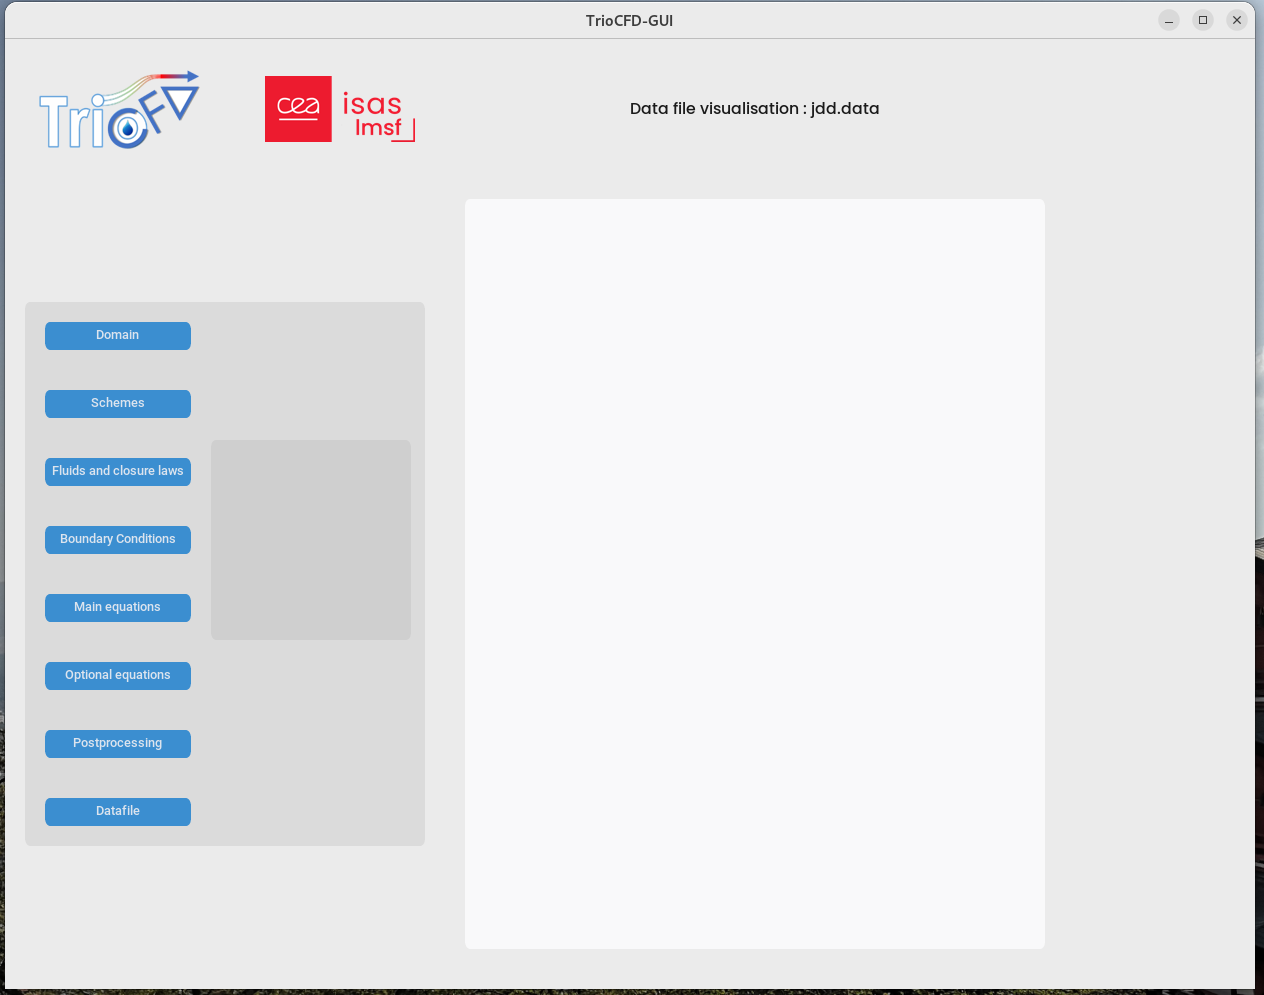
\includegraphics[scale=0.35]{Figure/GUI.png}
    \caption{Visualization of TrioCFD multiphase GUI.}
    \label{GUI}
\end{figure}
The GUI is coded in Python and may require the installation of the following packages: customtkinter, tkinter, and PIL. To launch the GUI, please find yourself in the right folder and do the command : python3 GUI. Its straightforward approach is based on reading and writing files, allowing users to fill in the data file step by step without loosing every files. Generally, users just need to click as many blue buttons as possible. However, red buttons should be used with caution. To complete the file, simply interact with all the buttons on the left side of the main interface. Don't forget to save at each submenu and to push the End datafile button when finished. The data file visualization window on the right is especially useful for checking that the data file is being filled out correctly.
\begin{figure}[htbp] 
\centering 
\begin{subfigure}[b]{0.45\textwidth} 
\centering 
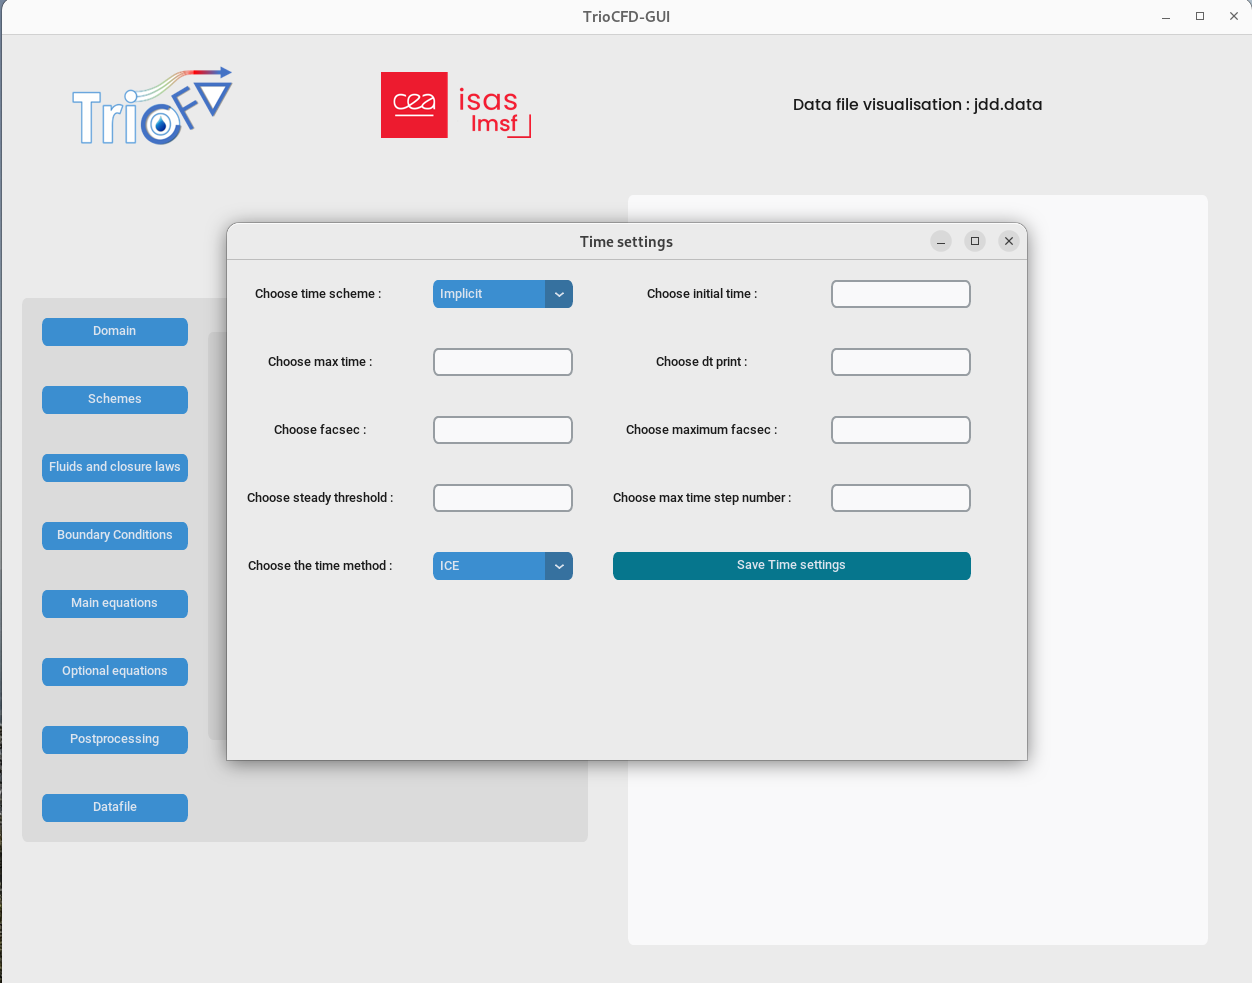
\includegraphics[scale=0.2]{Figure/Guitime.png} 
\caption{Time settings of GUI.}  
\end{subfigure} 
\hfill 
\begin{subfigure}[b]{0.45\textwidth} 
\centering 
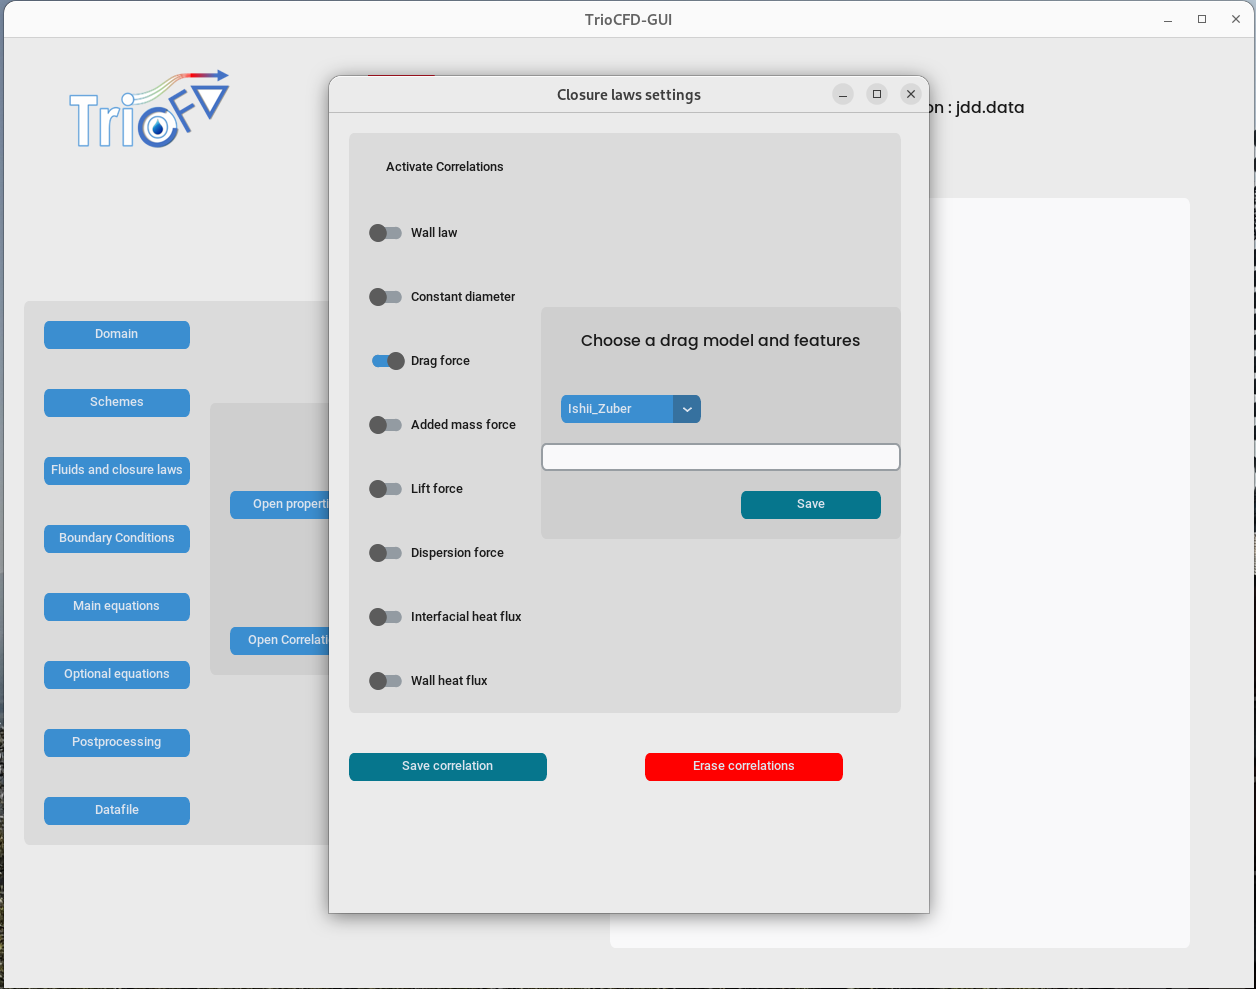
\includegraphics[scale=0.2]{Figure/Guicorrel.png} 
\caption{Closure laws of GUI.} 
 \end{subfigure} \\[1ex] 
\begin{subfigure}[b]{0.45\textwidth} 
\centering 
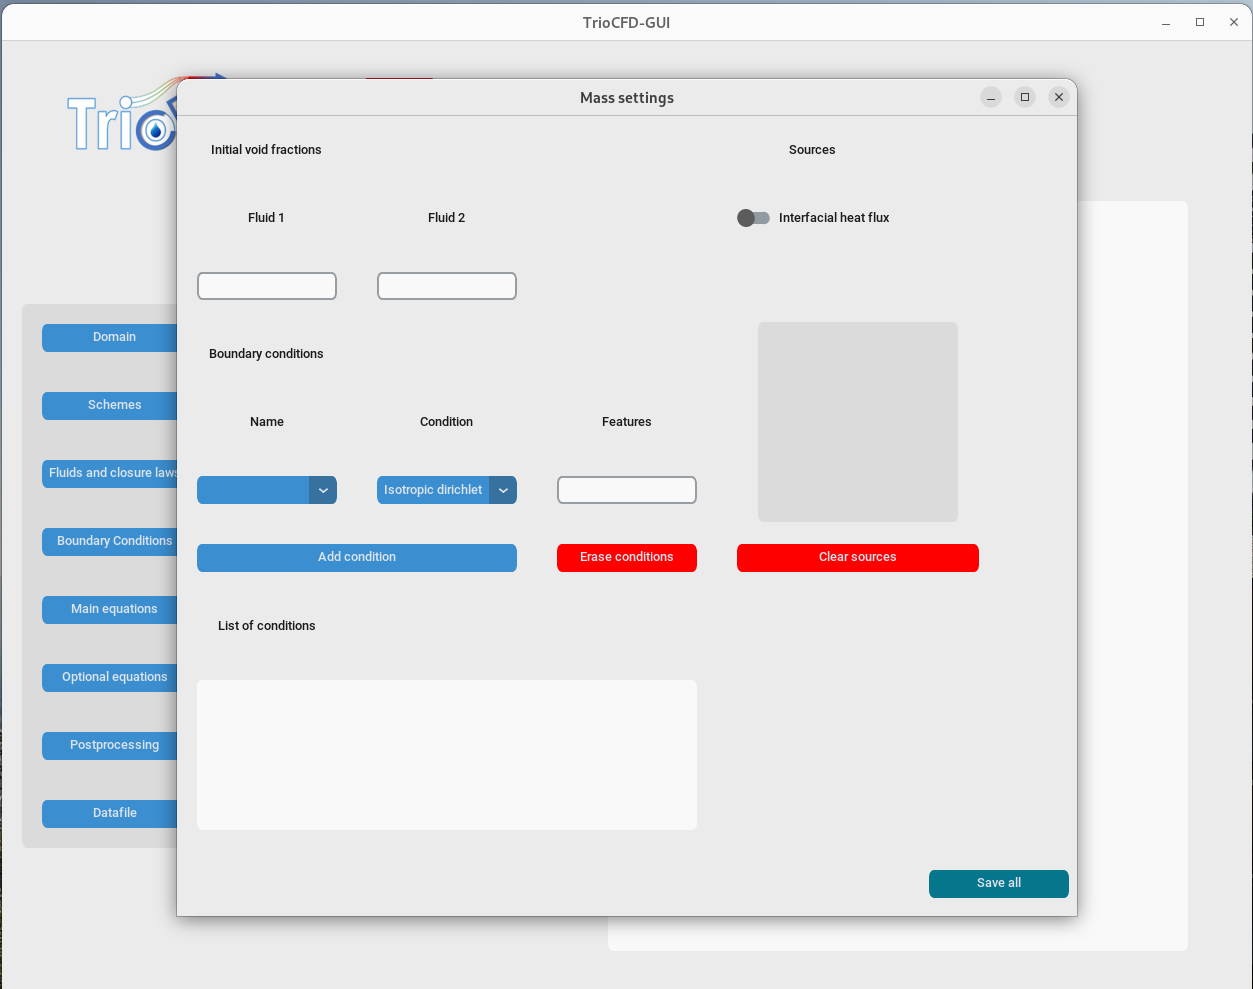
\includegraphics[scale=0.2]{Figure/Guimass.png} 
\caption{Mass equation settings of GUI.} 
\end{subfigure} \hfill 
\begin{subfigure}[b]{0.45\textwidth} 
\centering 
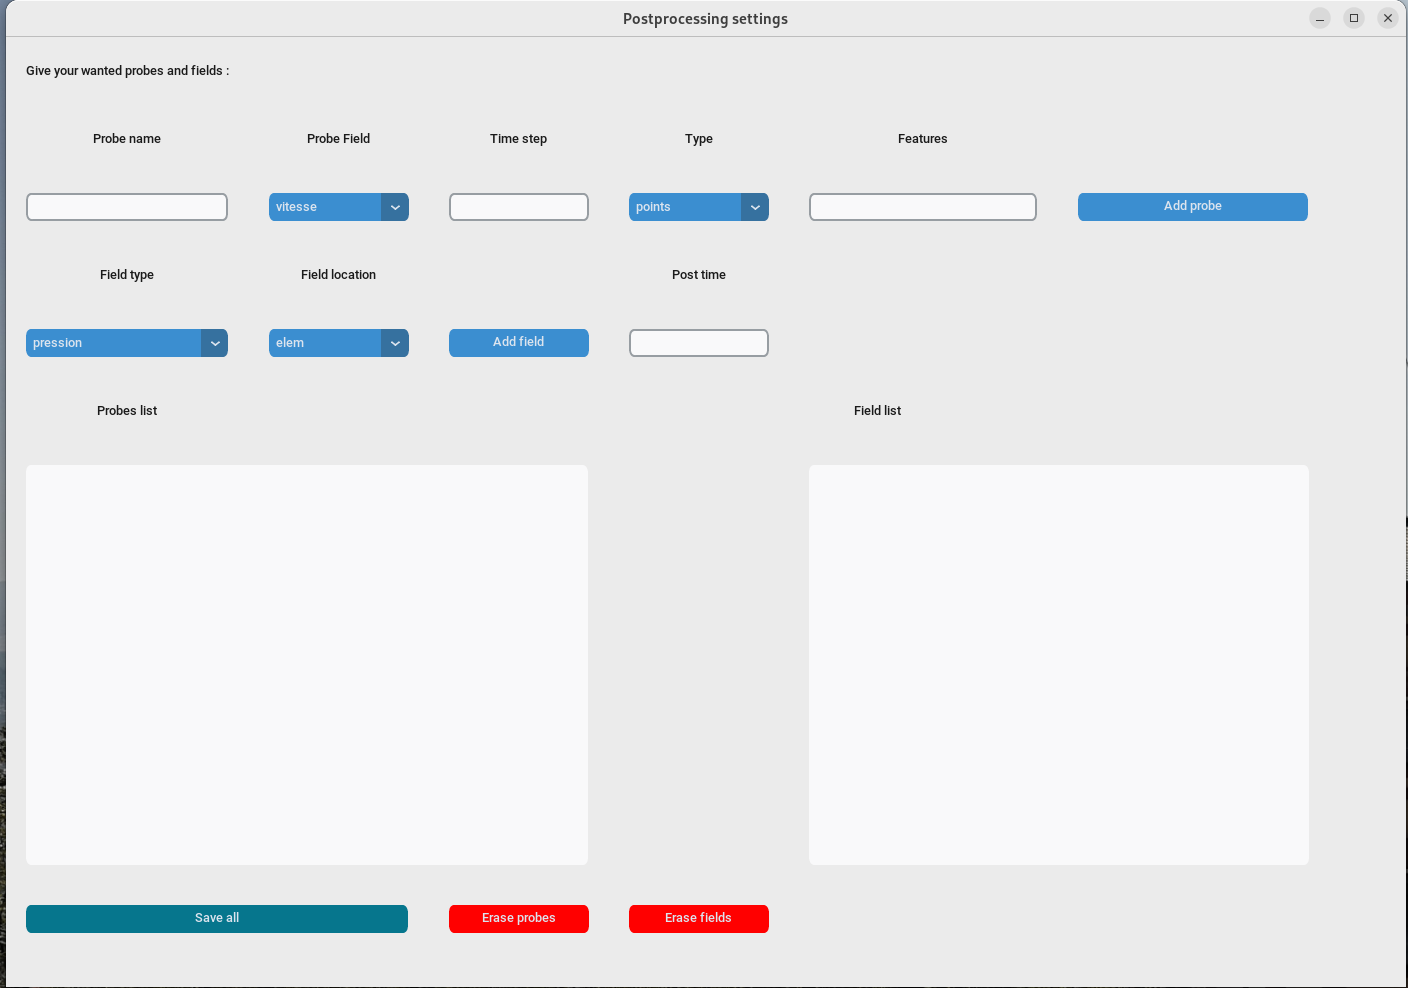
\includegraphics[scale=0.175]{Figure/Guipost.png} 
\caption{Post-processing settings of GUI.}  
\end{subfigure} 
\caption{Snapshots of different sub-menus of the GUI.}  
\end{figure} 